% !TeX program = lualatex
% Standalone wrapper: renders the original magnetic Aharonov--Bohm TikZ figure
% (../notes/figures/a-bohm-solenoid.tex) for the dark reveal.js deck.
% The figure source is NOT duplicated here: colours are remapped so that the
% notes and the slides stay a single source of truth.
\documentclass[tikz,border=2pt]{standalone}

\usepackage{fontspec}
\setmainfont{STIX Two Text}
\usepackage{unicode-math}
\setmathfont{STIX Two Math}

\usetikzlibrary{arrows.meta,angles,quotes,calc,decorations.markings}

% --- deck palette (talk/theme.scss) ---
\definecolor{paper}{HTML}{DCE3EC}
\definecolor{night}{HTML}{070D17}
\definecolor{accent}{HTML}{F2C94C}

% Remap the two base colours used by the figure instead of editing it:
%   black -> light ink on the dark background
%   white -> background, so the open vertex markers stay "open"
\colorlet{black}{paper}
\colorlet{white}{night}

\begin{document}
\color{paper}
% Aharonov--Bohm magnetic setup: TikZ fragment included from main.tex.
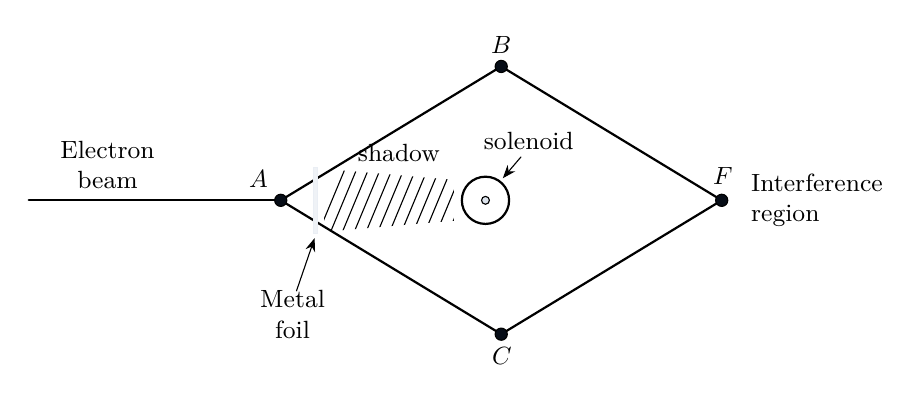
\begin{tikzpicture}[>=Stealth, line cap=round, font=\small]

	% ---- coordinate principali ----
	\coordinate (A) at (0,0);      % punto di separazione (foil)
	\coordinate (B) at (2.8,1.7);  % vertice superiore
	\coordinate (C) at (2.8,-1.7); % vertice inferiore
	\coordinate (F) at (5.6,0);    % regione di interferenza
	\coordinate (S) at (2.6,0);    % solenoide

	% ---- fascio incidente ----
	\draw[thick] (-3.2,0) -- (A);
	\node[align=center] at (-2.2,0.45) {Electron\\ beam};

	% ---- cammini del "rombo" ----
	\draw[thick] (A) -- (B) -- (F);
	\draw[thick] (A) -- (C) -- (F);

	% ---- lamina metallica (metal foil) ----
	\draw[fill=black!45, draw=black!60, line width=0.3pt]
	(0.42,-0.42) rectangle (0.47,0.42);
	\draw[->] (0.2,-1.15) -- (0.43,-0.48);
	\node[align=center] at (0.15,-1.45) {Metal\\ foil};

	% ---- zona d'ombra (shadow) ----
	\begin{scope}
		\clip (0.55,0.40) -- (2.2,0.26) -- (2.2,-0.26) -- (0.55,-0.40) -- cycle;
		\foreach \x in {0.4,0.55,...,2.3}
		\draw[thin] (\x,-0.6) -- (\x+0.5,0.6);
	\end{scope}
	\node at (1.5,0.60) {shadow};

	% ---- solenoide ----
	\draw[thick] (S) circle (0.30);
	\draw[fill=black] (S) circle (0.05);
	\node at (3.15,0.75) {solenoid};
	\draw[->] (3.05,0.55) -- (2.82,0.28);

	% ---- vertici (piccoli cerchi aperti) ----
	\foreach \p/\pos in {A/above left, B/above, C/below}{
			\draw[fill=white] (\p) circle (2.2pt);
			\node[\pos=1pt] at (\p) {$\p$};
		}

	% ---- regione di interferenza ----
	\draw[fill=white] (F) circle (2.2pt);
	\node[above=2pt] at (F) {$F$};
	\node[align=left, anchor=west] at (5.85,0) {Interference\\ region};

\end{tikzpicture}

\end{document}
